\section{Introduction}\label{sec:intro}

\emph{Structure editors}
have long promised to improve the programming experience
for beginners and experts alike.
By eliminating parse errors,
they provide cognitive benefits for novices
  \cite{meta-analysis-blocks,blocks-text-high-school,coblox}
  and end-users
  \cite{weitnauer2016graspable,rousillon,BasHermans21};
  simplify language composition
  \cite{mbeddr}
  and language-aware editor tooling
  \cite{HazelnutSNAPL};
  and form an essential component of truly continuous live programming
  \cite{Hazelnut,HazelnutLive}.
Yet, in the forty years since the idea was first
introduced and implemented \cite{Cornell},
structure editing has failed to reach
mainstream use by programmers beyond the novice level.
The problem, as many have observed
\cite{user-modeling,fine-tuning-selection-semantics,
practical-lang-based-editing,lang-on-the-usefulness,
psg,Minor92,TowardUserFriendly,MillerPMV94},
is that structure editors can be too slow
or difficult to use.

For example, while
block-based editors like Scratch \cite{scratch}
excel at introducing programming
to children and end-users, they soon become unwieldy
as users gain experience and create larger programs.
Cited issues include their inefficient mouse-driven
input, low visual information density, and rigid
tree-based construction of operator sequences
\cite{BlocksFingertips,cog-dim-blocks,blocks-and-beyond,no-keyboard-cripples}.

Meanwhile, the JetBrains MPS \cite{DBLP:conf/icse/VoelterP12}
editor resolves those particular issues with
keyboard-driven text-like interfaces---and
is used regularly by some professional programmers---but
instead suffers from steep learning curves and difficult-to-predict
editing behavior.
Consider the violin plots in Figure \ref{fig:mps-violin-plots},
which show post-task questionnaire responses from
a controlled user study of MPS \cite{ProjEfficiency}.
The left two plots show that MPS novices felt that
selection was relatively slow and inaccurate despite
a 45-minute training session and another 30-45 minutes
worth of study tasks.
Meanwhile, the right two plots show that
MPS novices and \emph{experts} alike struggled to
predict the effects of deletion.

\begin{figure}[b]
  \centering
  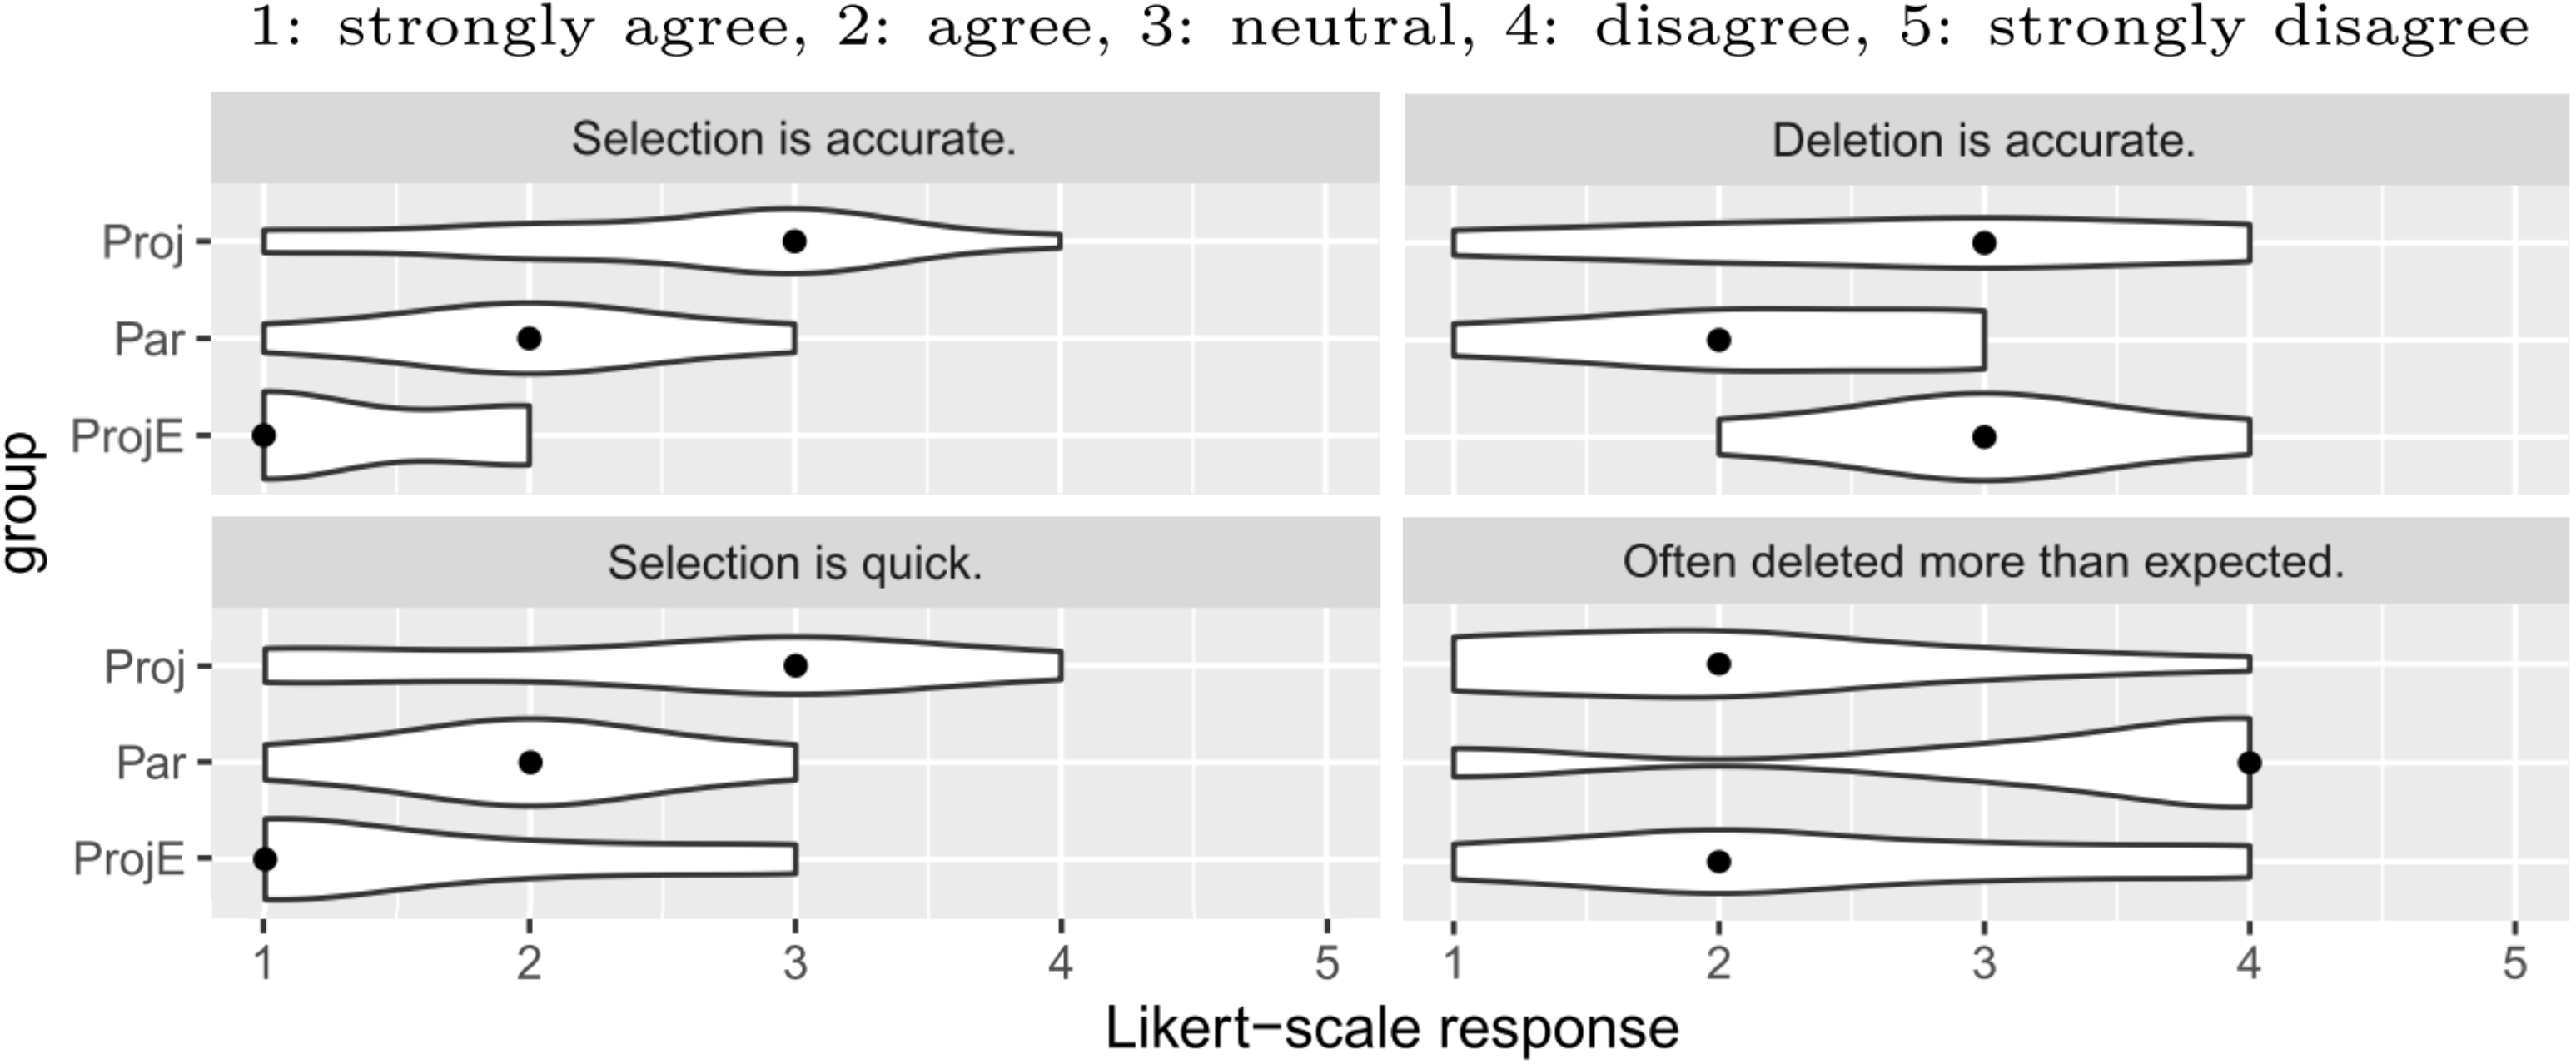
\includegraphics[width=\columnwidth]{img/mps-violin-plots.png}
  \caption{Violin plots of post-task questionnaire responses
  from a controlled user study of MPS, adapted from \cite{ProjEfficiency}.
  Each plot partitions the responses across the three study groups:
  novice MPS users (Proj), expert MPS users (ProjE),
  and text editor users (Par).
  }
  \label{fig:mps-violin-plots}
\end{figure}

Whether they are mouse-driven and block-based,
or keyboard-driven and text-like,
structure editors as a whole have suffered
from high viscosity \cite{cog-dim},
\ie, it is difficult to modify
and restructure existing code.
We believe this is a fundamental consequence
of the basic assumption that structure editors
should operate directly on the abstract syntactic structure
of a program.
% \footnote{\note{add comment here clarifying
% this is talking about pure structure editors and not
% hybrid ones and forward reference to related work}}
This assumption restricts selections to complete
program terms, a severe limitation compared to
the arbitrary range selections of text editors.
% \note{come back if there's time and talk a bit about
% Amy's thing and weave in a little more text editor vs
% structure editor dichotomy earlier}

In this paper, we describe a new approach to structure
editing, called \emph{tile-based editing}, that
recovers many of the flexible and linear editing
affordances of text editors.
The key insight is that, in order to guarantee edit state
well-formedness, it is sufficient to maintain a structure
more relaxed than the abstract syntactic structure demands,
but on which parsing is guaranteed to succeed.

Using a tile-based editor, the user manipulates
structural components called \emph{tiles} that
are shaped to fit together according to their
syntactic roles, \ala blocks in a block-based editor.
Unlike blocks, tiles directly model linear
operator sequences and facilitate left-to-right
editing using keyboard input.

Uniquely, tiles may be broken apart into
\emph{shards} as needed to specify arbitrary range
selections up to token boundaries.
Using a novel \emph{restructuring mode}, the user
may then ``cut and paste'' these selections like
in a text editor.
Unlike text-based cut-and-paste, restructuring
mode ensures you paste your selections such that
the result is a well-formed program term.

% Instead of representing the program in the language's
% abstract syntax, a tile-based editor represents it
% in a parallel tile-based syntax equipped with its own
% syntax-directed editing.

% Closely related to nested words \cite{nested-words}
% and visibly pushdown languages \cite{visibly-pushdown-langs},
% tiles encode both the linearity of sequentially
% positioned syntactic elements as well as
% their hierarchical nesting between matching sets
% of delimiters.

% \note{contributions: design and implementation of a
% minimal tile-based editor,
% formalization sketch of tile-based editing,
% discussion of how tile-based editing can be scaled up
% to more text-like interfaces like Hazel, plan to evaluate}

